\documentclass{article}
\usepackage{graphicx} % Required for inserting images
\usepackage{svg} % Makes it possible to include svg-images
\usepackage{cite}
\usepackage[a4paper, total={6in, 8in}]{geometry}

% --- Mathematics ---
\usepackage{bm}         % Bold text in math mode
\usepackage{amsmath}    % Math formulas and improved typographical quality of their output
\usepackage{amssymb}    % Extended symbol collection
\usepackage{amsthm}     % Helps define theorem-like structures
\usepackage{textcomp}   % Used in the package "gensymb" (below), which will give warnings if "textcomp" is not imported in advance
\usepackage{gensymb}    % Adds extra generic symbols for math and text mode, e.g. \degree

% --- Main matter ---
% This is the main part of the paper.
\newcommand{\mainmatter}{
    \newpage
    \pagenumbering{arabic}  % Setting page numbering to normal integers
}

\usepackage[colorlinks=true,allcolors=black]{hyperref}
\usepackage[british]{babel}     % Defining UK English as language. This will among other things ensure that dates are displayed as 24/03/1997 rather than 03/24/1997 in the bibliography.
\addto\extrasbritish{   % Change naming of different functions, e.g. figure references.
    \renewcommand*\contentsname{Table of Contents}  % Rename table of contents
    \renewcommand{\listfigurename}{List of Figures} % Rename list of figures
    \renewcommand{\listtablename}{List of Tables}   % Rename list of tables
    \def\equationautorefname{Equation}              % Autoref-name for equations
    \def\figureautorefname{Figure}                  % Autoref-name for figures
    \def\tableautorefname{Table}                    % Autoref-name for tables
    \def\sectionautorefname{Section}                % Autoref-name for sections
    \def\subsectionautorefname{Subsection} % Autoref-name for subsections
    \def\subsubsectionautorefname{Subsection} % Autoref-name for subsubsections
}

\begin{document}

\begin{titlepage}
\vbox{ }
\vbox{ }
\begin{center}
% Upper part of the page
\includesvg[width=\textwidth]{Figures/logo.svg}\\[1cm]
\textsc{\LARGE TFE4152 Design of Integrated Circuits}\\[1cm]
\textsc{\Large Term project fall 2024}\\[0.5cm]
\vbox{ }

% Title
{ \huge \bfseries 8x8-bit Memory System}\\[0.4cm] 

% Author
\large
\emph{Authors:}\\
L. Strand \& S.W. Kalland \\
Group 3
\vfill

\end{center}
\end{titlepage}

\begin{abstract}
    The abstract \textit{(Norwegian: sammendrag)} should sum up the key points of your report. It is good to include key details here (e.g. concrete numbers describing the design and/or results). In real life, many people stop reading after the abstract. This is your chance to present what your paper/report is all about, and to attract interest from the right readers.

    The abstract should answer the following questions:

    \quad What is this report all about?

    \quad What have you designed?

    \quad Why should I read this thesis?
    
    \quad What were the key results?

    Length: For a report this length, around half a page would probably be good. Maximum one page.
    
\end{abstract}
%\textit{This document shows the structure expected from your final reports. We follow the IMRaD structure, which you can read more about here: \url{https://writingcenter.gmu.edu/writing-resources/imrad/writing-an-imrad-report}.\\ IMPORTANT: You do not have to use \LaTeX, or even this specific \LaTeX-template. \textbf{What you must follow is the report structure presented in this document.}}.\\
%Briefly introduce your project. 
%The introduction should answer the following questions:
%\quad What is the problem?
%\quad What are your specifications?
%\quad How is the report structured? (E.g.: Results from simulations are presented in \autoref{sec:Results}).
\section{Introduction}
We are given an assignment to design a memory unit to be used in an IoT device. The memory unit is to have a total of 64 bit storage capacity. Furthermore, the system is to have a word length of 8 bit and a read / write time of no longer than \SI{3}{ns}.

All specifications are listed in the assignment sheet \cite{oppgavebeskrivelse}, with necessary theory presented in \autoref{sec:02:theory}. Our implementation of the solution is presented in \autoref{sec:03:method} with following results in \autoref{sec:04:results}. We will discuss our design in greater detail in \autoref{sec:05:discussion} and make some concluding remarks in \autoref{sec:06:conclusion}.
\section{Theory}    \label{sec:02:theory}

\subsection{Memory Unit}
Every digital memory unit is built up hierarchically by several word cells. The size of each word may vary from system to system (8-bit, 16-bit, 32-bit, etc.), but no matter the architecture, the smallest unit of memory, the bitcell, is present. The total available bits in the memory is the product of the number of bits per word times number of words in the unit. Every bit is addressable by a unique address that points to a single word in the unit. When reading or writing a word, the whole word is accessed, and should individual bits be of interest, then those must be parsed from the word.

The bitcells within each word are designed differently depending on the level of transparency required. There are several options for storing a single digital value, such as latches and flip-flops. Latches are transparent in the sense that once enabled, the output will follow the input immediately (with some negligible delay). Flip-flops on the other hand are not transparent: The output must always be overwritten by a rising or falling clock edge, thus delaying the output compared to the input.

\subsection{Power Reduction}
Total power consumption of a system is usually calculated as the sum of the static power consumption and the dynamic power consumption. The static power consumption is always present, even when the system is idle, meaning no inputs or outputs are changing. The dynamic power consumption is the extra power required to change the states of the system.

\begin{equation}
    P_{total} = P_{static} + P_{dynamic}
    \label{eq:02:total_power}
\end{equation}

Static power consumption is calculated by the average number of transistors that are in the active region, and how much each transistor leaks. The dynamic power consumption depends on many factors, but it can be reduced by lowering any of the system factors it is proportional to, see \autoref{eq:02:dynamic_power} \cite{forelesningslidesPower}.

\begin{equation}
    P_{dynamic} \propto f_{clk} \cdot C_{load} \cdot V_{DD}^2
    \label{eq:02:dynamic_power}
\end{equation}

In reason years, with clock frequencies going down, it is the static power consumption that contribute to the most of the over all power consumption, despite Moore's law. In order to reduce power consumption in a 'System on a Chip' (SoC) there are many factors to consider, but some very common ones are to: 
\begin{itemize}
    \item Reduce the number of transistors in the system as a whole.
    \item Reduce the current through each transistor when in the active region, which can be estimated with equation \ref{eq:02:drain_current} \cite{analog2011}. 
    \item Reduce supply voltage
    \item Reduce the switching frequency / clock frequency.
\end{itemize}


To reduce the drain current, some adjustments to the transistor specifications based on \autoref{eq:02:drain_current} can be made:
\begin{itemize}
    \item Reduce the width-to-length ratio.
    \item Minimize the difference between voltage supply and threshold voltage of the transistors.
\end{itemize}

To achieve the latter, one may choose to wither lower the voltage supply directly or increase the threshold voltage by tuning the bulk of each transistor. 


\begin{equation}
    I_D = \frac{\mu C_{ox}}{2} \frac{W}{L} (V_{GS} - V_T)^2 
    \label{eq:02:drain_current}
\end{equation}


\subsection{Process variation corners}
When producing SoC's, the transistors on the wavefer are prone to be slightly different from each other depending on a number of factors. Transistors made close together on the wavefer will be more similar to each other than transistors placed further apart. These process variations makes some transistors switch on and off faster than others. We divide the transistors into 5 different corners according to how fast they are switching.

\begin{itemize}
    \item \makebox[1cm]{FF \hfill} \makebox[2.5cm]{\textit{Fast-Fast} \hfill} Fast operating NMOS and Fast operating PMOS 
    \item \makebox[1cm]{SS \hfill} \makebox[2.5cm]{\textit{Slow-Slow} \hfill} Slow operating NMOS and Slow operating PMOS 
    \item \makebox[1cm]{FS \hfill} \makebox[2.5cm]{\textit{Fast-Slow} \hfill} Fast operating NMOS and Slow operating PMOS 
    \item \makebox[1cm]{SF \hfill} \makebox[2.5cm]{\textit{Slow-Fast} \hfill} Slow operating NMOS and Fast operating PMOS 
    \item \makebox[1cm]{TT \hfill} \makebox[2.5cm]{\textit{Typical-Typical} \hfill} Typical operating NMOS and Typical operating PMOS 
\end{itemize}

The advantages of fast operating transistors include faster switching times and lower threshold voltages, meaning that they can operate on a lower voltage supply. However they have higher power consumption due to the higher leakage current and switching frequency. The leakage current is a result of the shorter channel lengths meaning less capacitance between the channels. The lowered threshold voltage $V_T$ will also provide higher leakage current. When $V_T$ is lower, it means that even a small voltage at the gate can cause the transistor to start conducting, which also makes it more susceptible to unwanted or subthreshold leakage. Subthreshold leakage occurs when the gate voltage is below $V_T$, but still close enough to allow a small current to flow through the channel. In contrast to fast transistors, slow transistors have a higher $V_T$ and thus lower power consumption, which makes them ideal for low energy implementations.

\section{Method}
\subsection{System overview}

%TODO: add figure of system diagram (FSM + RAM):
\begin{figure}
    \centering
    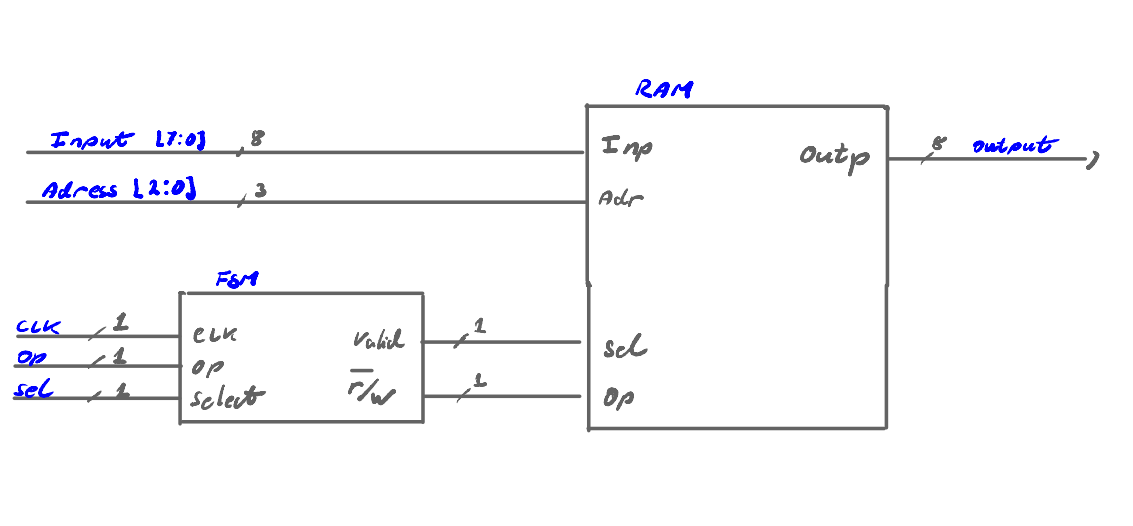
\includegraphics[width=0.8\linewidth]{LaTeX_2/Figures/memory_block_schematic.png}
    \caption{System diagram}
    \label{fig:03:system_diagram}
\end{figure}

Our system consists of a Finite State Machine and a Random Access Memory, as can be seen in \autoref{fig:03:system_diagram}. The FSM serves as a control unit to make sure all operations on the RAM are performed in a stable manner. The FSM is connected to a clock signal, but the RAM is not directly, only indirectly through controll by the FSM.

%%%%%%%%%%%%%%%%%%%%%%%%%%%%%%%%%%%%%%%%%%%%%%%%%%%%%%%%%%%%%%%%%%%%%%%%%%%%%%%%%%%%%%%%%%%%%
%                                         RAM                                               %
%%%%%%%%%%%%%%%%%%%%%%%%%%%%%%%%%%%%%%%%%%%%%%%%%%%%%%%%%%%%%%%%%%%%%%%%%%%%%%%%%%%%%%%%%%%%%
\subsection{RAM}
The RAM subsystem consists of eight bitcells forming eight bytecells that stack on top of each other to form the full memory. It has these inputs and outputs:
\begin{itemize}
    \item \makebox[2cm]{adr \hfill} - 3-bit address signal
    \item \makebox[2cm]{inp \hfill} - 8-bit input data to be stored in address
    \item \makebox[2cm]{outp \hfill} - 8-bit output data to be read from address
    \item \makebox[2cm]{op \hfill} - either 0 for read or 1 for write
    \item \makebox[2cm]{sel \hfill} - must be 1 for op to affect the circuit
\end{itemize}

When the circuit is reading, meaning \textsc{op} is low, the output is what is stored in the currently addressed bytecell. When it is writing, the outp is Z (high resistance), meaning it can be easily overwritten, and should not be trusted. We chose our output to be Z as that seemed like the clearest solution, since it is necessary for the circuit to be in read mode in order to be read from.

The RAM's circuit is as in \autoref{fig:03:RAM_schematic}. It consists of eight bytecell modules. Each of the output busses is connected together as it is only possible to read from one of the bytecell modules at a time.

\begin{figure}
    \centering
    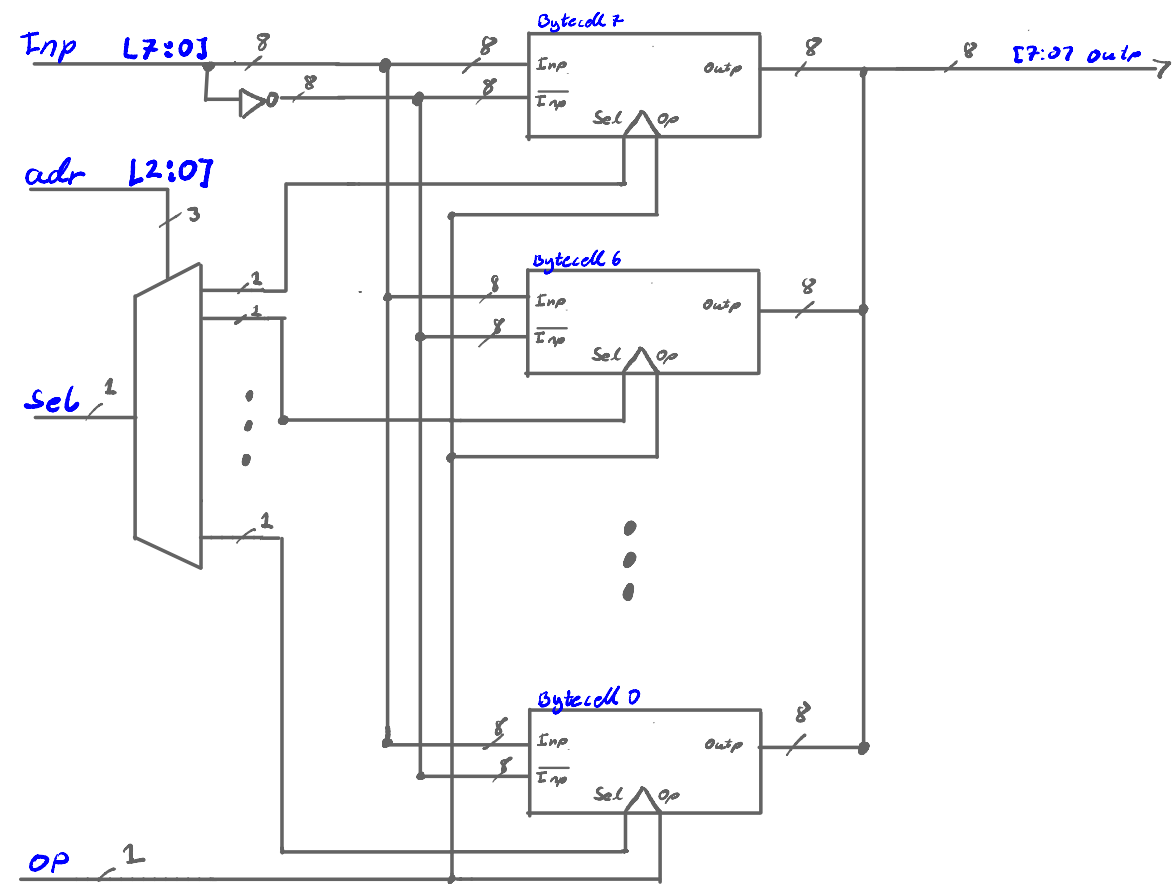
\includegraphics[width=0.8\linewidth]{LaTeX_2/Figures/ram_schematic.png}
    \caption{Full schematic for the RAM subsystem}
    \label{fig:03:RAM_schematic}
\end{figure}


%%%%%%%%%%%%%%%%%%%%%%%%%%%%%%%%%%%%%%%%%%%%%%%%%%%%%%%%%%%%%%%%%%%%%%%%%%%%%%%%%%%%%%%%%%%%%
%                                         BITCELL                                           %
%%%%%%%%%%%%%%%%%%%%%%%%%%%%%%%%%%%%%%%%%%%%%%%%%%%%%%%%%%%%%%%%%%%%%%%%%%%%%%%%%%%%%%%%%%%%%
\subsubsection{The bitcell}
The bitcell concists of a D-latch and a tri-state-buffer. The logic schematic of the D-latch, connected to the transistor schematic of a tri-state-buffer, can be seen in \autoref{fig:03:bitcell_schematic}.

\begin{figure}[H]
    \centering
    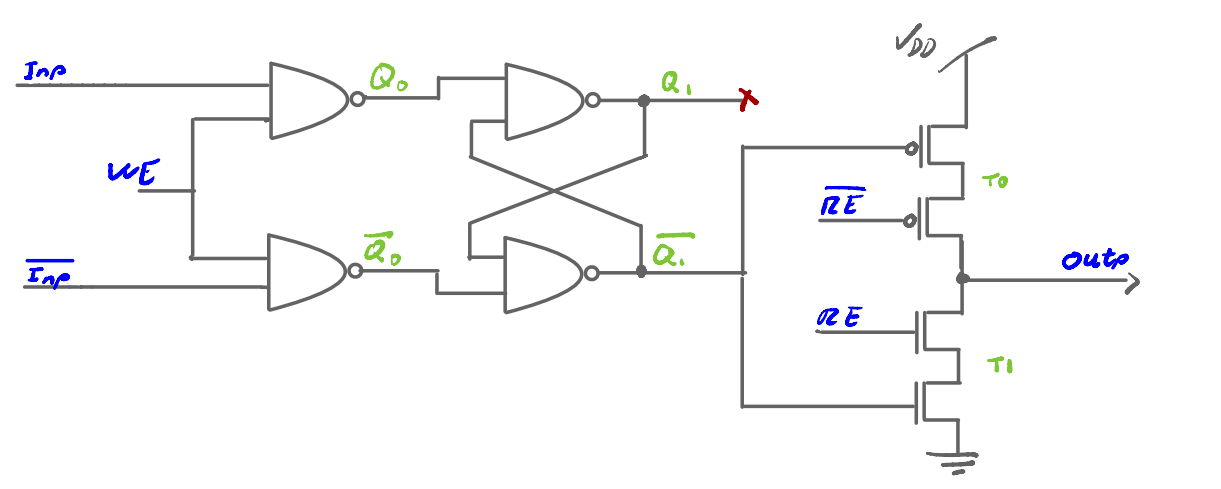
\includegraphics[width=0.8\linewidth]{LaTeX_2/Figures/bitcell_schematic.png}
    \caption{Wiring schematic for the bitcell module}
    \label{fig:03:bitcell_schematic}
\end{figure}

The bitcell has inputs and outputs:
\begin{itemize}
    \item \makebox[2cm]{inp \hfill} - The input bit to be stored
    \item \makebox[2cm]{inpn \hfill} - (input not) The inverse of the input bit
    \item \makebox[2cm]{outp \hfill} - The output when the circuit is read
    \item \makebox[2cm]{WE \hfill} - Write Enable, must be high to store a new value
    \item \makebox[2cm]{RE \hfill} - Read Enable, must be high to set outp to the stored value
\end{itemize}

The stored value sits in $\overline{Q_1}$, since the tri-state buffer acts as an iverter. We choose to implement the bitcell with a tri-state-buffer in order to make the output high impedance ($Z$) when \textsc{RE} is low. This is to ensure that the common bus in the RAM module can be overwritten by the selected bytecell module if \textsc{RE} is active.
This simplifies the rest of the design, since there is no need for a multiplexer to choose which address to read data from. 

\hspace{}

The leakage current of each bitcell are a sum of the leakage current of all the transistors that make up one bitcell. In total there are 20 transistors in each bitcell, 10 \textsc{NMOS} and 10 \textsc{PMOS}. The leakage current of one \textsc{NMOS} can be estimated from equation \ref{eq:03:leakage_current}
TODO: Bitcell analog properties. W, L, VDD




%%%%%%%%%%%%%%%%%%%%%%%%%%%%%%%%%%%%%%%%%%%%%%%%%%%%%%%%%%%%%%%%%%%%%%%%%%%%%%%%%%%%%%%%%%%%%
%                                         BYTECELL                                          %
%%%%%%%%%%%%%%%%%%%%%%%%%%%%%%%%%%%%%%%%%%%%%%%%%%%%%%%%%%%%%%%%%%%%%%%%%%%%%%%%%%%%%%%%%%%%%
\subsubsection{The bytecell}
The bytecell consists of 8 bitcells and an F-block (function block) meant to translate the input signals of the bytecell to the required inputs of each of its bitcells. The bitcells all write their outputs to 8 different wires, which we refer to as the data bus. The bytecell can be seen in \autoref{fig:03:bytecell_schematic}.

\begin{figure}[H]
    \centering
    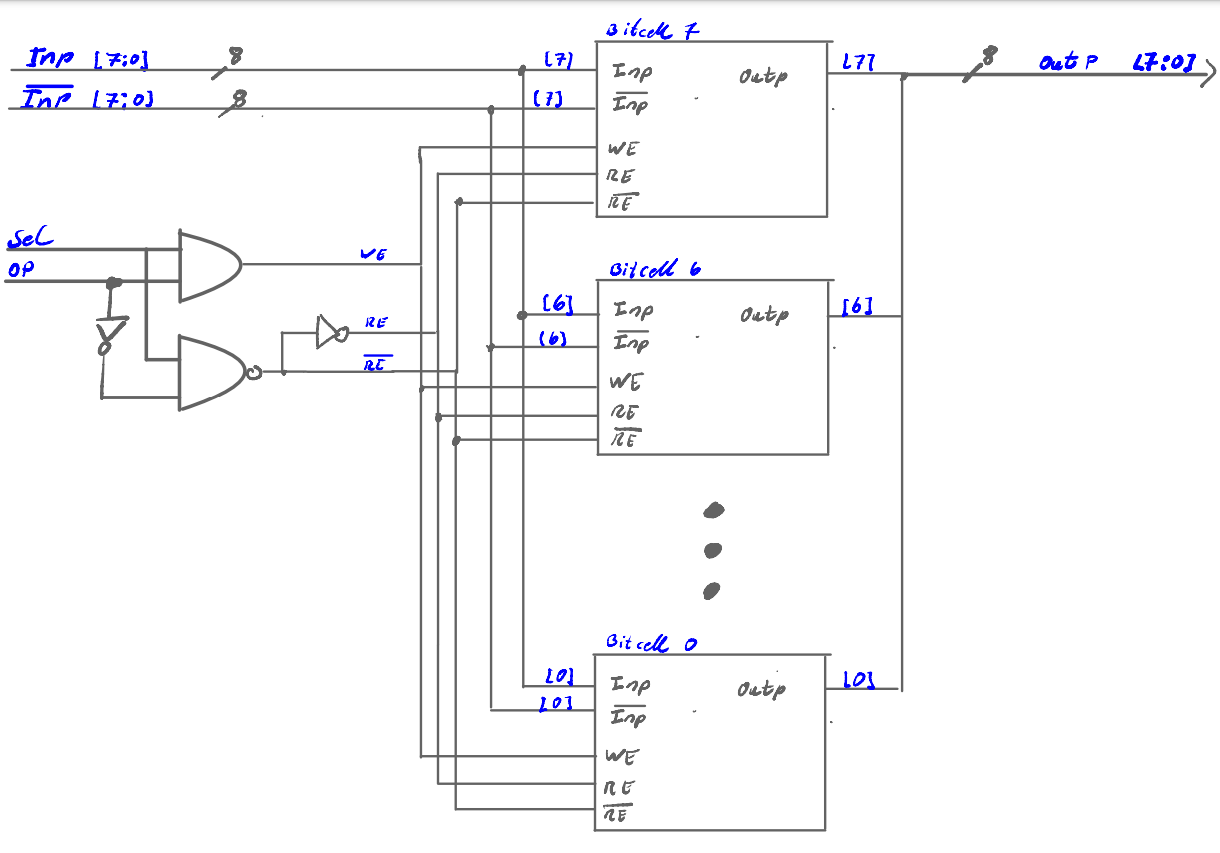
\includegraphics[width=0.8\linewidth]{LaTeX_2/Figures/bytecell_schematic.png}
    \caption{Wiring schematic for the bytecell module}
    \label{fig:03:bytecell_schematic}
\end{figure}

The inputs and outputs of the bytecell are almost identical to those of the RAM, with the exception of there being no address signal, and the input having to be written both normally and inverted. Having the inverse signal at this level means saving transistors, as there will be one inverter for each of the 8 data bus wires one level higher, instead of one inverter for every bitcell.

The F-block was designed to set WE high only when op and sel are high, and to set RE high only when op is low and sel is high, and otherwise to set both WE and RE to low.


%%%%%%%%%%%%%%%%%%%%%%%%%%%%%%%%%%%%%%%%%%%%%%%%%%%%%%%%%%%%%%%%%%%%%%%%%%%%%%%%%%%%%%%%%%%%%
%                                         FMS                                               %
%%%%%%%%%%%%%%%%%%%%%%%%%%%%%%%%%%%%%%%%%%%%%%%%%%%%%%%%%%%%%%%%%%%%%%%%%%%%%%%%%%%%%%%%%%%%%
\subsection{FSM}
The finite state machine is meant to work as an interface for stable use of the RAM subsystem. Together they make up the memory system. It was designed by looking at the state diagram, \autoref{fig:03:state_diagram}, from the project task. Then proceeding by giving code values to each of the states, \autoref{tab:03:state_code}, setting up a truth table, \autoref{tab:03:FSM_truth_table}, and using the logical relations between the inputs, outputs, current state and next state, \autoref{eq:03:boolean_equation}, to design a typical FSM circuit, \autoref{fig:03:FSM_schematic}.


The transistor circuit implementation of the D-latch in the bitcell can be seen in \autoref{fig:03:D-latch_schematic}.

%TODO: add figure of transistor circuit for the D-latch
\begin{figure}[H]
    \centering
    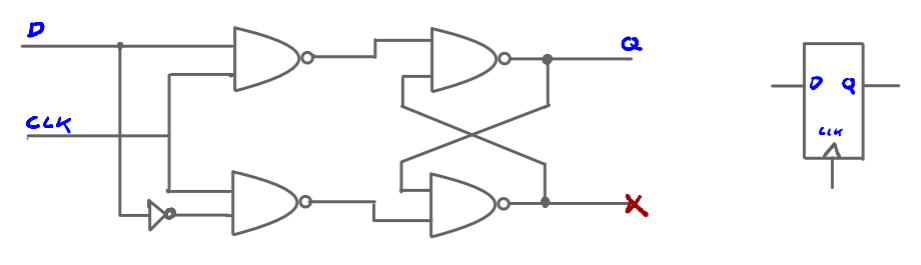
\includegraphics[width=0.8\linewidth]{LaTeX_2/Figures/flipflop.png}
    \caption{Circuit schematic of the D-latch in the bitcell}
    \label{fig:03:D-latch_schematic}
\end{figure}


\begin{figure}
    \centering
    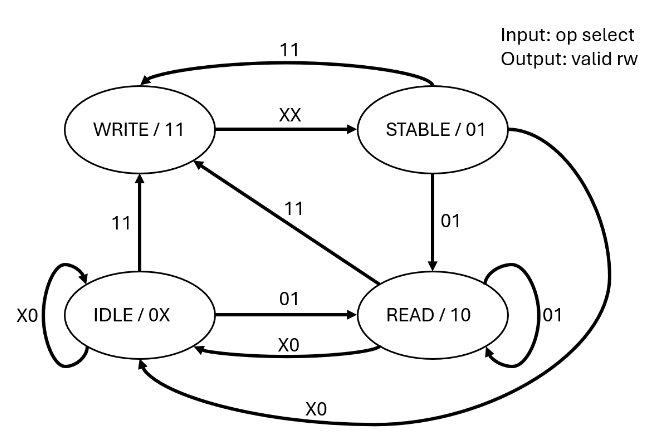
\includegraphics[width=0.8\linewidth]{LaTeX_2/Figures/state_diagram.png}
    \caption{Desired state diagram \cite{oppgavebeskrivelse}}
    \label{fig:03:state_diagram}
\end{figure}

\begin{table}[]
    \caption{State code and their meaning.}
    \centering
    \begin{tabular}{|l|c|}
        \hline
        State   &   Code    \\  \hline
        IDLE    &   0 X     \\  
        STABLE  &   0 1     \\
        READ    &   1 0     \\
        WRITE   &   1 1     \\  \hline
    \end{tabular}
    \label{tab:03:state_code}
\end{table}

\subsubsection{Circuit design}
\begin{figure}
    \centering
    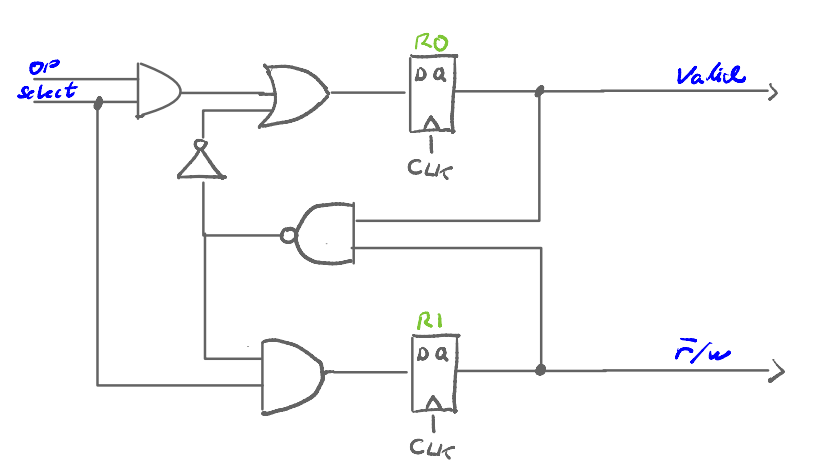
\includegraphics[width=0.8\linewidth]{LaTeX_2/Figures/fsm_schematic.png}
    \caption{Wiring schematic for the FSM logic.}
    \label{fig:03:FSM_schematic}
\end{figure}

\begin{table}[]
    \caption{Truth table for Finite State Machine.}
    \centering
    \begin{tabular}{|cc|cc|cc|cc|}
        \hline
        \multicolumn{2}{|l|}{State} & \multicolumn{2}{l|}{Input} & \multicolumn{2}{l|}{State nxt} & \multicolumn{2}{l|}{Output}        \\ \hline
                     &              & Op          & Sel          &                &               & Valid & R/W \\
        A            & B            & C           & D            & E              & F             & G     & H                          \\ \hline
        0            & 0            & 0           & 0            & 0              & X             & 0     & X                          \\
        0            & 0            & 0           & 1            & 1              & 0             & 0     & X                          \\
        0            & 0            & 1           & 0            & 0              & X             & 0     & X                          \\
        0            & 0            & 1           & 1            & 1              & 1             & 0     & X                          \\
        0            & 1            & 0           & 0            & 0              & X             & 1     & 0                          \\
        0            & 1            & 0           & 1            & 1              & 0             & 1     & 0                          \\
        0            & 1            & 1           & 0            & 0              & X             & 1     & 0                          \\
        0            & 1            & 1           & 1            & 1              & 1             & 1     & 0                          \\
        1            & 0            & 0           & 0            & 0              & X             & 0     & 1                          \\
        1            & 0            & 0           & 1            & 1              & 0             & 0     & 1                          \\
        1            & 0            & 1           & 0            & 0              & X             & 0     & 1                          \\
        1            & 0            & 1           & 1            & 1              & 1             & 0     & 1                          \\
        1            & 1            & 0           & 0            & 0              & 1             & 1     & 1                          \\
        1            & 1            & 0           & 1            & 0              & 1             & 1     & 1                          \\
        1            & 1            & 1           & 0            & 0              & 1             & 1     & 1                          \\
        1            & 1            & 1           & 1            & 0              & 1             & 1     & 1                          \\ \hline
    \end{tabular}
    \label{tab:03:FSM_truth_table}
\end{table}



\begin{equation}
\begin{split}
    E   &=  D \cdot \overline{A \cdot B}\\
    F   &=  A \cdot B + C \cdot D       \\
    G   &=  B                           \\
    H   &=  A
\end{split}
    \label{eq:03:boolean_equation}
\end{equation}


\section{Simulations and Results}\label{sec:Results}
Present the results of your simulations in this section. Use tables and graphs or other figures to illustrate your results. Remember: The table caption goes above the table, the figure caption goes below the figure.

For each test/simulation, make sure to answer the following: 

\quad Why are you doing this test? 

\quad Can you describe the testbench? E.g. applied stimuli, the circuit being tested etc.

\quad What were the results? Use figures and/or tables to present them. 

\quad Are the results as expected / within spec? \textit{NOTE: This is not the place to discuss why the results are as they are, that should be saved for the discussion-section.}
\section{Discussion}
Discuss your results. You presented your results in the last section, so you do not need to repeat everything here. Just focus on the most interesting results and discuss these.

Was there anything unexpected or weird about your results? What are possible explanations for these observations? It is good to draw on theory. This section and the theory section are the sections where it is natural to have the most references to literature (papers, the book, other).

The discussion section should aim to cover the following:

\quad If the circuit did not work properly, \textit{why} might that be? 

\quad If some of your results turn out differently than you expected: \textit{Why}? You do not have to come to a definite answer, but should try to discuss at least one possible explanation.

\quad Are there any parts of your implementation you would do differently, given another chance?

\quad It could be interesting to discuss the choices you made to reduce static power consumption, and potential improvements to these.


\textbf{Finally, your boss wants to send your design off to your colleague, so that they can create the circuit layout. Are you ready to give the "good to go"-signal, or are there changes or tests you would like to do first?}
\section{Conclusion}
Make some concluding remarks. The length of this section should be somewhere between a paragraph and a page.

The conclusion should include your key findings. Make the conclusion as concrete as possible by using numbers for the result (e.g. what was the static power consumption at a given supply voltage).

You should answer the following:

\quad What did you achieve?

\quad Does this align with what you set out to achieve at the start?

\quad Are there any particular results you want to highlight?


\newpage
\addcontentsline{toc}{section}{References}
\bibliographystyle{unsrt}
\bibliography{bibliography}

\newpage
\vspace*{7 cm}
\begin{center}
\textbf{\Huge Appendices}
\end{center}
\addcontentsline{toc}{section}{Appendices}
\appendix
\section{AIMSpice Code}
Include all your AIMSpice code here. You might want to include snippets of it earlier in the text as well, but the entire code should at least be included here.
\\ \\
Remember to format and comment your code for increased readability.

\section{Verilog Code}
Include all your verilog code here. You might want to include snippets of it earlier in the text as well, but the entire code should at least be included here.
\\ \\
Remember to format and comment your code for increased readability.


\section{Optional (rename based on what you put here)}
Sometimes one might end up running a lot of simulations, and then find out that not all of them were relevant enough to present in the actual report. Additional figures and results can then be included here (with a brief explanation so that the reader knows what they are looking at). This section of the appendix is optional, and might not be relevant for your group. 

Anything added here will not affect the grade directly, but might contribute to the overall impression of the work you have done (which is part of what we grade). Your grade will NOT be affected negatively if only the AIMSpice and Verilog code is in the appendix.
\end{document}
